\documentclass{article}
\usepackage[T1]{fontenc}
\usepackage{lmodern}
\usepackage{graphicx}
\usepackage{amsmath,amssymb}
\usepackage[a4paper,margin=2cm]{geometry}
\usepackage[absolute,overlay]{textpos}
\setlength{\TPHorizModule}{1mm}
\setlength{\TPVertModule}{1mm}
\usepackage[indonesian]{babel}
\usepackage{hyperref}
\setlength{\emergencystretch}{2em}
% unit: Halaman 35

\begin{document}

% === Halaman 35 (llm) ===

\vspace{44.55mm}

\begin{itemize}
    \item Kunci adalah string: $K = k_1 k_2 \dots k_m$
    $k_i$ untuk $1 \le i \le m$ menyatakan huruf-huruf alfabet
    
    \item Jika panjang kunci lebih pendek daripada panjang plainteks, maka kunci diulang secara periodik.
    
    \item Misalkan panjang kunci $m = 10$, maka 10 huruf pertama plainteks dienkripsi dengan kunci $K$, setiap huruf ke-$i$ menggunakan kunci $k_i$.
\end{itemize}

\vspace{10mm}

Contoh: kunci = \texttt{soreang} \quad (dalam angka: $18, 14, 17, 4, 0, 13, 6$)

\begin{tabular}{ll}
Plainteks: & \texttt{terimapesanangulaikambing} \\
Kunci: & \texttt{soreangsoreangsoreangsore}
\end{tabular}

\vspace{5mm}

Untuk 8 karakter berikutnya, kembali menggunakan pola enkripsi yang sama.

% deskripsi: Tabel pemetaan huruf alfabet ke angka dari A=0 sampai Z=25
% bbox normalisasi: [0.5300, 0.0000, 0.9800, 0.1500]
\begin{textblock*}{94.50mm}(111.30mm,0.00mm)
\noindent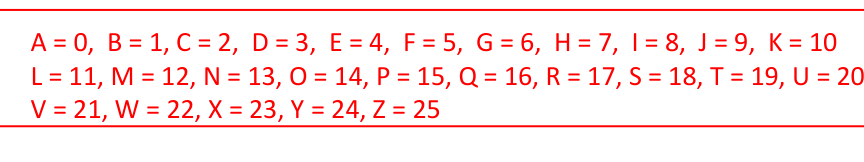
\includegraphics[width=94.50mm,height=44.55mm]{../../images/llm/page_035_img_01.png}%
\end{textblock*}

% deskripsi: Kotak penjelasan yang menyatakan bahwa setiap huruf plainteks dienkripsi menggunakan Caesar Cipher dengan kunci k yang berbeda-beda
% bbox normalisasi: [0.6300, 0.6700, 0.9800, 0.8100]
\begin{textblock*}{73.50mm}(132.30mm,198.99mm)
\noindent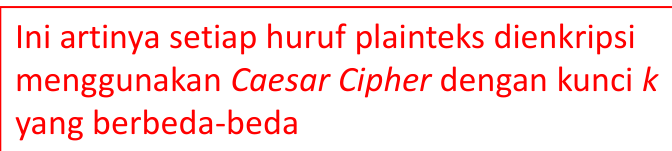
\includegraphics[width=73.50mm,height=41.58mm]{../../images/llm/page_035_img_02.png}%
\end{textblock*}

\end{document}
